

\documentclass{beamer}
\usetheme{Frankfurt}
\usecolortheme{dove}
\usepackage{graphicx}
\usepackage{xcolor}
\usepackage{multicol}
\newcommand\indep{\protect\mathpalette{\protect\independenT}{\perp}}
\def\independenT#1#2{\mathrel{\rlap{$#1#2$}\mkern2mu{#1#2}}}
\definecolor{dblue}{RGB}{0,0,139}
\usepackage{tikz}
\usetikzlibrary{arrows,shapes.arrows,positioning,shapes,shapes.misc}
\usetikzlibrary{decorations.pathreplacing}
\usepackage{booktabs}
\renewcommand{\arraystretch}{1.2}
\newcommand{\Cov}{\text{Cov}}
\newcommand{\E}{{\mathbb{E}}}
\newcommand{\Var}{\text{Var}}
\newcommand{\V}{\mathbb{V}}
\renewcommand{\P}{\mathbb{P}}
\usepackage{hanging}% http://ctan.org/pkg/hanging
\setbeamertemplate{footnote}{%
  \hangpara{2em}{1}%
  \makebox[2em][l]{\insertfootnotemark}\footnotesize\insertfootnotetext\par%
}
\newcommand{\myfootnote}{\let\thefootnote\relax\footnote}
\newcommand{\blue}[1]{\textcolor{blue}{#1}}
\newcommand{\green}[1]{\textcolor{olive}{#1}}
\newcommand{\purple}[1]{\textcolor{purple}{#1}}

\setbeamertemplate{footnote}{%
  \footnotesize\insertfootnotetext\par%
}
\usepackage{colortbl}
\newcommand{\argmin}[1]{\underset{#1}{\text{arg\,min }}}
\newcommand{\nospace}[1]{\makebox[0pt]{\hspace{6pt}#1}}

\title{Causal forests: A tutorial in high-dimensional causal inference}

\author{Ian~Lundberg}

%\institute[Princeton University] % (optional, but mostly needed)
%{
 % Department of Sociology and Office of Population Research\\
  %Princeton University}

\date{General Exam in Frontiers of Causal Inference\\ 12 October 2017}

\begin{document}

\section{Intro}

\begin{frame}

\begin{columns}
\begin{column}{0.55\textwidth}
\begin{center}\begin{huge}
\textcolor{blue}{Causal forests}\vskip .1cm 
\end{huge} \vskip .2cm \begin{large}
A tutorial in high-dimensional causal inference
\end{large}
 \vskip .5cm
Ian Lundberg \vskip .3cm
General Exam\\Frontiers of Causal Inference \vskip .2cm
12 October 2017
\end{center}
\end{column}
\begin{column}{0.45\textwidth}
\vskip 1.5cm
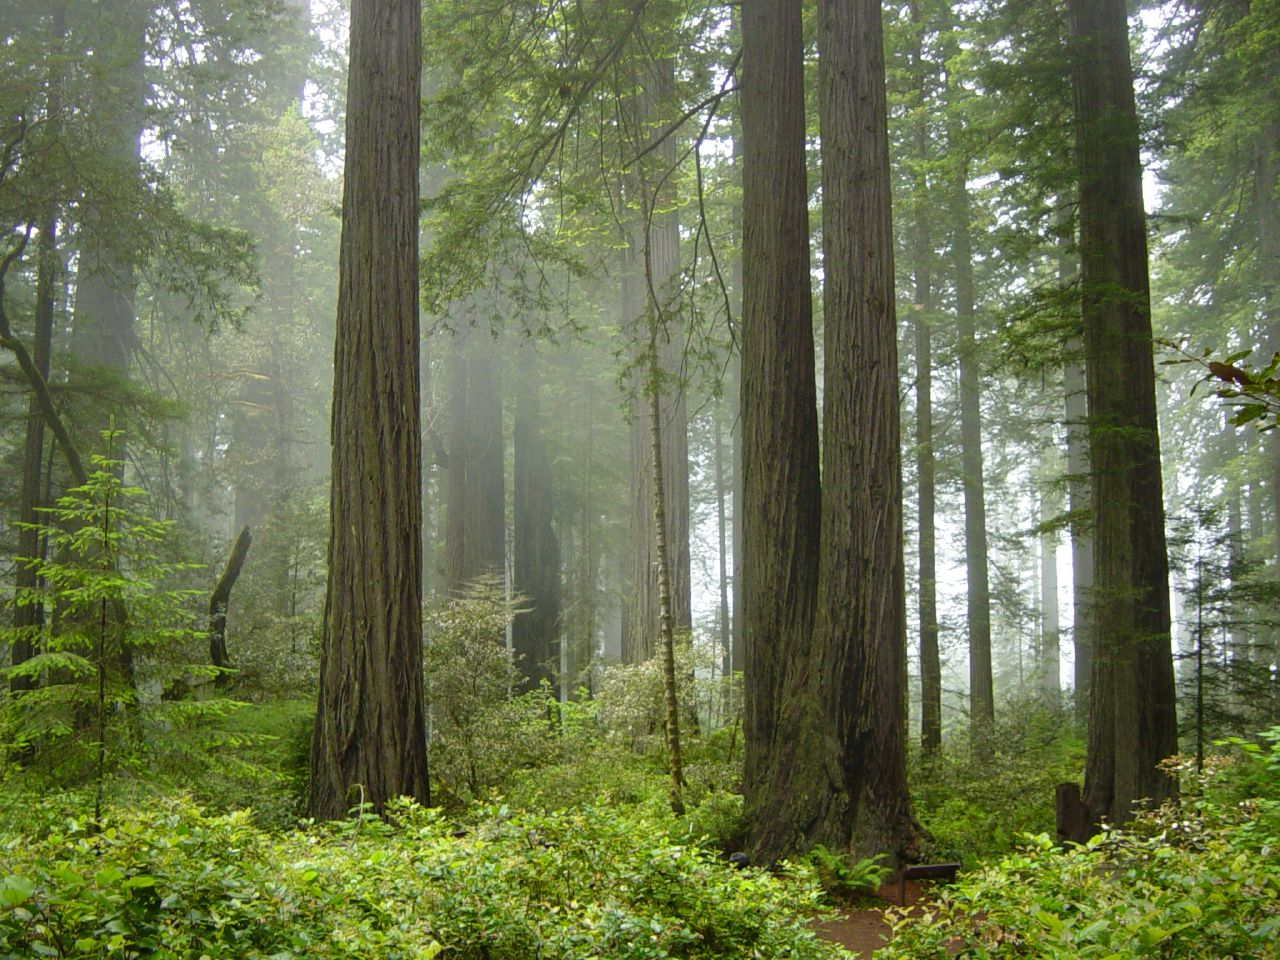
\includegraphics[width=\textwidth]{figures/Redwood} \\
\begin{footnotesize}PC: \href{https://commons.wikimedia.org/w/index.php?curid=4049158}{Michael Schweppe via Wikimedia Commons}\\ CC BY-SA 2.0\end{footnotesize}
%\begin{tikzpicture}[x = .7cm, y = 2cm]
%  \node (origin) at (0,0) {O};
%  \node (p1) at (-2,-1) {1};
%  \node (p2) at (2,-1) {2};
%  \draw[->, thick] (origin) -- (p1);
%  \draw[->, thick] (origin) -- (p2);
%  \end{tikzpicture}
 \end{column}
\end{columns}

\end{frame}

\begin{frame}{Introductory note for those finding these slides online}
These slides were prepared for the \href{https://scholar.princeton.edu/bstewart/sociology-statistics-reading-group}{Sociology Statistics Reading Group} at Princeton. Everyone read the following paper in advance:
\begin{quote}\normalfont
Athey, Susan, and Guido Imbens. 2016. Recursive partitioning for heterogeneous causal effects. \emph{Proceedings of the National Academy of Sciences}, 113(27):7353--7360. \blue{\href{https://www.pnas.org/content/113/27/7353.short}{[link]}}
\end{quote}
The aim was to discuss this paper so that together the group would leave with a good understanding of its contribution. Along the way, these slides touch on other related literature that uses tree-based methods for causal inference. In addition, these slides counted as one of several requirements for a general exam I completed in causal inference. \vskip .2cm
Disclaimer that I invented nothing in these slides, and there are likely places where I misread the original papers.
\end{frame}

\section{Potential outcomes}

\begin{frame}
\centering
\huge Note: These slides assume \
\blue{randomized} treatment assignment \\
until the section labeled ``confounding.''
\end{frame}

\begin{frame}{Causal inference: A missing data problem}
\begin{center}
\begin{tikzpicture}
\node at (0,0) {
\begin{scriptsize}
\begin{tabular}{cccccc}
& & & \multicolumn{2}{c}{Potential employment} & \\
\cmidrule(lr){4-5}
& Education & Treated & No job training & Job training & Treatment effect \\
ID & $X_i$ & $W_i$ & $Y_i(0)$ & $Y_i(1)$ & $\tau_i = Y_i(1) - Y_i(0)$ \\
\hline
1 & High school & 0 & \only<1-2>{0}\only<3->{0} & \only<1-2>{1}\only<3->{?} & \only<1-2>{1}\only<3->{?} \\
2 & High school & 1 & \only<1-2>{0}\only<3->{?} & \only<1-2>{1}\only<3->{1} & \only<1-2>{1}\only<3->{?} \\
3 & College &        0 & \only<1-2>{1}\only<3->{1}  & \only<1-2>{1}\only<3->{?} & \only<1-2>{0}\only<3->{?} \\
4 & College &        1 & \only<1-2>{1}\only<3->{?} & \only<1-2>{1}\only<3->{1} & \only<1-2>{0}\only<3->{?} \\
\end{tabular}
\end{scriptsize}
};
\only<2-2>{
\node[anchor=north] at (0,-2) {$\begin{aligned}
{\bar\tau} &= \bar{Y}_{i:W_i=1}(1) - \bar{Y}_{i:W_i=0}(0) \\
&= 1 - 0.5 \\
&= 0.5
\end{aligned}$};
}
\onslide<4-4>{
\node[anchor=north west] at (-5,-2) {If $W_i\indep \{Y_i(0),Y_i(1)\}$, then};
\node[anchor=north] at (0,-3) {$\begin{aligned}
\hat{\bar\tau} &= \bar{Y}_{i:W_i=1} - \bar{Y}_{i:W_i=0} \\
&= 1 - 0.5 \\
&= 0.5
\end{aligned}$};
}
\onslide<5-5>{
\node[anchor=north west] at (-5,-2) {What if we want to study $\tau_i=f(X_i)$?};
\node[anchor=north west] at (-5,-2.5) {\scalebox{.8}{$\begin{aligned}
\hat{\bar\tau}_\text{High school} &= \bar{Y}_{i:W_i=1,X_i=\text{High school}} \\
&\qquad - \bar{Y}_{i:W_i=0,X_i=\text{High school}} \\
&= 1 - 0.5 \\
&= 0.5
\end{aligned}$}};
\node[anchor=north east] at (5,-2.5) {\scalebox{.8}{$\begin{aligned}
\hat{\bar\tau}_\text{College} &= \bar{Y}_{i:W_i=1,X_i=\text{College}} \\
&\qquad - \bar{Y}_{i:W_i=0,X_i=\text{College}} \\
&= 1 - 1 \\
&= 0
\end{aligned}$}};
}
\onslide<6-8>{
\node at (0,-2) {What if there are dozens of $X$ variables?};
\onslide<7-8>{\node at (0,-2.5) {What if $X$ is continuous?};}
\onslide<8-8>{
\node at (0,-3.5) {It's hard to know \blue{which subgroups of $X$}};
\node at (0,-4) {might show interesting \blue{effect heterogeneity}};
}
}
\end{tikzpicture}
\end{center}
\end{frame}

\section{Algorithm}

\begin{frame}
\centering
\LARGE Start with a simpler \blue{prediction} question. \vskip 1cm
Which subgroups of $X$ have very different \blue{average outcomes?}
\end{frame}

\begin{frame}{Prediction: One tree}
\centering
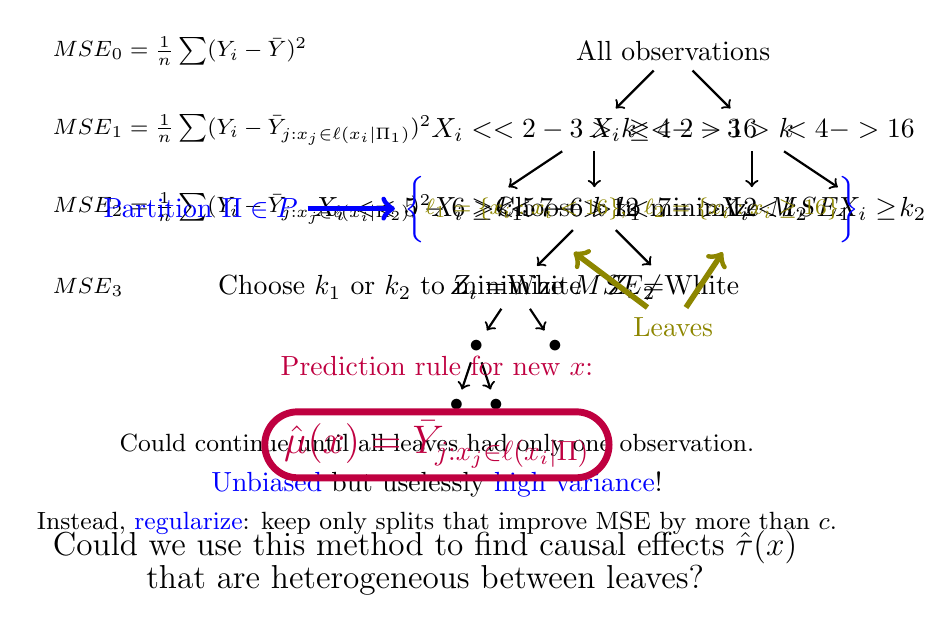
\begin{tikzpicture}
\node[anchor=west] at (-8,0) {\begin{footnotesize}$\text{MSE}_0 = \frac{1}{n}\sum (Y_i-\bar{Y})^2$\end{footnotesize}};
\node (head) at (0,0) {All observations}; \pause
\node[anchor=west] at (-8,-1) {\begin{footnotesize}$\text{MSE}_1 = \frac{1}{n}\sum (Y_i-\bar{Y}_{j:x_j\in\ell(x_i\mid \Pi_1)})^2$\end{footnotesize}};
\node (left) at (-1,-1) {$X_i < \onslide<2-3>{\nospace{$k$}}\onslide<4->{16}$};
\node (right) at (1,-1) {$X_i \geq \onslide<2-3>{\nospace{$k$}}\onslide<4->{16}$};
\draw[->, thick] (head) -- (left);
\draw[->, thick] (head) -- (right);
\onslide<3-3>{\node at (0,-2) {Choose $k$ to minimize $\text{MSE}_1$};}
\onslide<5-12>{
\onslide<5->{
\node (ll) at (-2.5,-2) {$X_i < \onslide<5-6>{\nospace{$k_1$}}\onslide<7->{12}$};
\node (lr) at (-1,-2) {$X_i \geq \onslide<5-6>{\nospace{$k_1$}}\onslide<7->{12}$};
\draw[->, thick] (left) -- (ll);
\draw[->, thick] (left) -- (lr);
\node[anchor=west] at (-8,-2) {\begin{footnotesize}$\text{MSE}_2 = \frac{1}{n}\sum (Y_i-\bar{Y}_{j:x_j\in\ell(x_i\mid \Pi_2)})^2$\end{footnotesize}};
}
}
\onslide<5-6>{
\node (rl) at (1,-2) {$X_i < \nospace{$k_2$}$};
\node (rr) at (2.5,-2) {$X_i \geq \nospace{$k_2$}$};
\draw[->, thick] (right) -- (rl);
\draw[->, thick] (right) -- (rr);
}
\onslide<6-6>{\node at (-3,-3) {Choose $k_1$ or $k_2$ to minimize $\text{MSE}_2$};}
\onslide<8-11>{
\node[anchor=west] at (-8,-3) {\footnotesize $\text{MSE}_3$};
%\node (lll) at (-3,-3) {$\bullet$};
%\node (llr) at (-2,-3) {$\bullet$};
\node (lrl) at (-2, -3) {$Z_i = $White};
\node (lrr) at (0,-3) {$Z_i \neq $White};
%\draw[->, thick] (ll) -- (lll);
%\draw[->, thick] (ll) -- (llr);
\draw[->, thick] (lr) -- (lrl);
\draw[->, thick] (lr) -- (lrr);
}
\onslide<9-10>{
%\node[anchor=west] at (-8,-4) {\footnotesize $\text{MSE}_4$};
\node (lrll) at (-2.5, -3.75) {$\bullet$};
\node (lrlr) at (-1.5, -3.75) {$\bullet$};
\draw[->, thick] (lrl) -- (lrll);
\draw[->, thick] (lrl) -- (lrlr);
\node (lrlll) at (-2.25, -4.5) {$\bullet$};
\node (lrllr) at (-2.75, -4.5) {$\bullet$};
\draw[->, thick] (lrll) -- (lrlll);
\draw[->, thick] (lrll) -- (lrllr);
}
\onslide<10-13>{
\node at (-3,-5) {\small Could continue until all leaves had only one observation.};
\node at (-3,-5.5){\blue{Unbiased} but uselessly \blue{high variance}!};
\node at (-3,-6) {\small Instead, \blue{regularize}: keep only splits that improve MSE by more than $c$.};
}
\onslide<14->{
\node[olive] (l1) at (-2,-2) {\footnotesize $\blue{\bigg\{}\ell_1=\{x_i:x_i < 16\},$};
\node[olive] (l2) at (1,-2) {\footnotesize $\ell_2=\{x_i:x_i \geq 16\}\blue{\bigg\}}$};
\node[blue] (partition) at (-6,-2) {Partition $\Pi\in\P$};
\draw[->, line width = 2pt, blue] (partition) -- (l1);
%\draw[line width = 2.5pt, blue,rounded corners=10pt] (-2,-2.5) rectangle (2,-3.5);
\node[olive] (leaves) at (0,-3.5) {Leaves};
\draw[->, line width = 2pt, olive] (leaves) -- (l1);
\draw[->, line width = 2pt, olive] (leaves) -- (l2);
}
\onslide<15->{
\node[purple] at (-3,-4) {Prediction rule for new $x$:};
\node[purple,line width = 2.5pt,rounded rectangle,draw] at (-3,-5) {\Large $\hat\mu(x) = \bar{Y}_{j:x_j\in\ell(x_i\mid \Pi)}$};
}
\onslide<16->{
\node[anchor=west,align=center] at (-8,-6.5) {\large Could we use this method to find causal effects $\hat\tau(x)$ \\\large that are heterogeneous between leaves?};
}
\end{tikzpicture}
\end{frame}

\begin{frame}{Causal tree: What's different?}
\begin{enumerate}
\item We do not observe the ground truth \pause
\item Honest estimation:
\begin{itemize}
\item One sample to choose partition
\item One sample to estimate leaf effects
\end{itemize} \pause
\end{enumerate}
\blue{Why is the split critical?} \vskip .2cm
Fitting both on the training sample risks \blue{overfitting}: Estimating many ``heterogeneous effects'' that are really just noise idiosyncratic to the sample. \vskip .2cm \pause
\begin{center}\begin{Large}We want to search for true heterogeneity, not noise.\end{Large}\end{center}
\end{frame}

\section{Sample split}

\begin{frame}{Sample splitting}
$$\text{MSE}_\mu(S^\text{te},S^\text{est},\Pi) \equiv \frac{1}{\#(S^\text{te})}\sum_{i\in S^\text{te}}\bigg\{\overbrace{(Y_i-\hat\mu(X_i;S^\text{est},\Pi))^2}^\text{MSE criterion} - \overbrace{Y_i^2}^{\substack{\text{Authors add}}}\bigg\}$$ \pause
$$\text{EMSE}_\mu(\Pi) \equiv \E_{S^\text{te},S^\text{est}}\bigg[\text{MSE}_\mu(S^\text{te},S^\text{est},\Pi)\bigg]$$ \pause
\blue{Honest criterion}: Maximize
\begin{center}
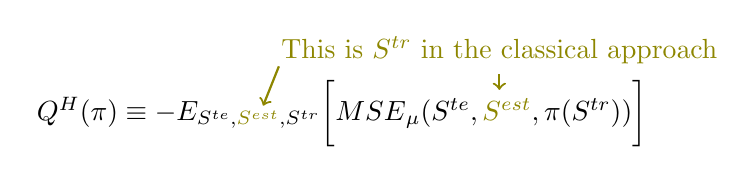
\begin{tikzpicture}
\node at (0,0) {$Q^H(\pi) \equiv -\E_{S^\text{te},\green{S^\text{est}},S^\text{tr}}\bigg[\text{MSE}_\mu(S^\text{te},\green{S^\text{est}},\pi(S^\text{tr}))\bigg]$};
\node[olive] (classic) at (2,.8) {This is $S^\text{tr}$ in the classical approach};
\draw[->, thick, olive] (classic) -- (2,.3);
\draw[->, thick, olive] (-.8,.6) -- (-1,0.1);
\end{tikzpicture}
\end{center}
where $\pi:\mathbb{R}^{p+1}\rightarrow \P$ is a function that takes a training sample $S^\text{tr}\in\mathbb{R}^{p+1}$ and outputs a partition $\Pi\in\P$.

\myfootnote{Note: The authors include the final $Y_i^2$ term to simplify the math; it just shifts the estimator by a constant.}
\end{frame}

\begin{frame}{Analytic estimator for $\text{EMSE}_\mu(\Pi)$ (p. 7356)}
\begin{center}
\Large \blue{Goal}: Estimate expected MSE using only the training sample. \vskip 1cm
This will be used to place splits when training a tree.
\end{center}
\end{frame}

\begin{frame}{Analytic estimator for $\text{EMSE}_\mu(\Pi)$ (p. 7356)}
\begin{center}
\begin{tikzpicture}
\node at (0,0) {\scalebox{.7}{$\begin{aligned}
-\text{EMSE}_\mu(\Pi) &= -\E_{S^\text{te},S^\text{est}}\Bigg[\bigg(Y_i - \hat\mu(X_i\mid S^\text{est},\Pi)\bigg)^2-Y_i^2\Bigg] \\
\\
&= \only<1-4>{-\E_{S^\text{te},S^\text{est}}\Bigg[\bigg(Y_i - \mu(X_i\mid\Pi) + \mu(X_i\mid\Pi) - \hat\mu(X_i\mid S^\text{est},\Pi)\bigg)^2-Y_i^2\Bigg]}
\only<5-5>{-\E_{S^\text{te},S^\text{est}}\Bigg[\bigg(Y_i\green{{}- \mu(X_i\mid\Pi) + \mu(X_i\mid\Pi)} - \hat\mu(X_i\mid S^\text{est},\Pi)\bigg)^2-Y_i^2\Bigg]}
\only<6->{-\E_{S^\text{te},S^\text{est}}\Bigg[\bigg(\blue{Y_i - \mu(X_i\mid\Pi)} + \green{\mu(X_i\mid\Pi) - \hat\mu(X_i\mid S^\text{est},\Pi)}\bigg)^2-Y_i^2\Bigg]} \\
\\
&= -\E_{S^\text{te},S^\text{est}}
\only<1-5>{\Bigg[\bigg(Y_i - \mu(X_i\mid\Pi)\bigg)^2-Y_i^2\Bigg]}
\only<6->{\blue{\Bigg[\bigg(Y_i - \mu(X_i\mid\Pi)\bigg)^2-Y_i^2\Bigg]}}  \\
\\
&\qquad -\E_{S^\text{te},S^\text{est}}
\only<1-5>{\Bigg[\bigg(\mu(X_i\mid\Pi) - \hat\mu(X_i\mid S^\text{est},\Pi)\bigg)^2\bigg]} 
\only<6->{\green{\Bigg[\bigg(\mu(X_i\mid\Pi) - \hat\mu(X_i\mid S^\text{est},\Pi)\bigg)^2\bigg]}}\\
\\
&\qquad -\E_{S^\text{te},S^\text{est}}\Bigg[2
\only<1-4>{\bigg(Y_i - \mu(X_i\mid\Pi)\bigg)}
\only<5->{\blue{\bigg(Y_i - \mu(X_i\mid\Pi)\bigg)}}
\only<1-4>{\bigg(\mu(X_i\mid\Pi) - \hat\mu(X_i\mid S^\text{est},\Pi)\bigg)}
\only<5->{\green{\bigg(\mu(X_i\mid\Pi) - \hat\mu(X_i\mid S^\text{est},\Pi)\bigg)}}
\Bigg] \\
\end{aligned}$}};
\onslide<2-4>{
\node (n1) at (-3.4,3.3) {\tiny \blue{Expected mean squared error for a partition $\Pi$}};
\draw[->,thick,blue] (n1) -- (-3.4,2.9);
}
\onslide<3-4>{
\node (n2) at (-2,2) {\tiny \blue{Over estimation sets used to estimate the leaf-specific $\hat\mu$ and test sets to evaluate those}};
\draw[->,thick,blue] (n2) -- (-2,2.5);
}
\onslide<4-4>{
\node (n3) at (2,3.3) {\tiny\green{Prediction based on $S^\text{est}$ from the leave $\ell(X_i)$ containing $X_i$}};
\draw[->,thick,olive] (0,3.2) -- (0,2.9);
}
\onslide<5-5>{
\node (n4) at (0, 2.2) {\green{Add a zero}};
\draw[->,thick,olive] (n4) -- (0,1.6);
\draw[->,thick,olive] (n4) -- (1.3,1.6);
}
\onslide<6-6>{
\node (n5) at (-2,.7) {\blue{First term${}^2$}};
\draw[->,blue,thick] (-1,1.1) -- (-.5,.5);
\node (n6) at (3.5,.5) {\green{Second term${}^2$}};
\draw[->,olive,thick] (2.5,1.1) -- (1.2,-.7);
\node (n7) at (1,-2) {\footnotesize 2\blue{(First term)}\green{(Second term)}};
}
\onslide<7-8>{
\node at (0,-2) {\blue{A}};
\node at (3,-2) {\green{B}};
\draw[->, thick, blue] (0,-2.2) -- (0, -2.5);
\draw[->, thick, olive] (3,-2.2) -- (3, -2.5);
\node[align=left,anchor=west] at (-6.2, -1) {\tiny $E(A)=0$ by assumption};
\node[align=left,anchor=west] at (-6.2, -1.75) {\tiny $Cov(A,B)=0$ because $Y_i$ is from};
\node[align=left,anchor=west] at (-6.2, -2.1) {\tiny a sample independent of $S^\text{est}$};
\node[align=left,anchor=west] at (-6.2, -2.8) {\tiny $\begin{aligned}Cov(AB) &= E(AB) - E(A)E(B)\\0 &= E(AB) - 0\end{aligned}$};
}
\onslide<8-8>{
\node (zero) at (4, -1.85) {\huge $=0$};
\draw[->, line width = 2.5pt] (-2,-2.9) -- (zero);
}
\end{tikzpicture}
\end{center}
\end{frame}

\begin{frame}
\begin{center}
\begin{tikzpicture}
\node at (0,0) {\scalebox{.7}{$\begin{aligned}
&=-\E_{(Y_i,X_i),S^\text{est}}\bigg[(Y_i-\mu(X_i\mid\Pi))^2 - Y_i^2\bigg] \\
&\qquad-\E_{X_i,S^\text{est}}\bigg[(\hat\mu(X_i\mid S^\text{est},\Pi)-\mu(X_i\mid\Pi))^2\bigg] \\
\\
&=-\E_{(Y_i,X_i),S^\text{est}}\bigg[Y_i^2+\mu^2(X_i\mid\Pi) - 2Y_i\mu(X_i\mid\Pi) - Y_i^2\bigg] \\
&\qquad-\E_{X_i,S^\text{est}}\bigg[(\hat\mu(X_i\mid S^\text{est},\Pi)-\mu(X_i\mid\Pi))^2\bigg] \\
\\
&=
\only<1-3>{-\E_{(Y_i,X_i),S^\text{est}}\bigg[\mu^2(X_i\mid\Pi) - 2\mu(X_i\mid\Pi)\mu(X_i\mid\Pi)\bigg]}
\only<4-4>{\blue{{}-\E_{(Y_i,X_i),S^\text{est}}\bigg[\mu^2(X_i\mid\Pi) - 2\mu(X_i\mid\Pi)\mu(X_i\mid\Pi)\bigg]}} \\
&\qquad
\only<1-3>{-\E_{X_i,S^\text{est}}\bigg[(\hat\mu(X_i\mid S^\text{est},\Pi)-\mu(X_i\mid\Pi))^2\bigg]}
\only<4-4>{\green{{}-\E_{X_i,S^\text{est}}\bigg[(\hat\mu(X_i\mid S^\text{est},\Pi)-\mu(X_i\mid\Pi))^2\bigg]}} \\
\\
&=
\only<1-3>{\E_{X_i}\bigg[\mu^2(X_i\mid\Pi)\bigg] - \E_{S^\text{est},X_i}\bigg[\V(\hat\mu(X_i\mid S^\text{est},\Pi))\bigg]}
\only<4-4>{\blue{\E_{X_i}\bigg[\mu^2(X_i\mid\Pi)\bigg]}\green{{} - \E_{S^\text{est},X_i}\bigg[\V(\hat\mu(X_i\mid S^\text{est},\Pi))\bigg]}}
\end{aligned}$}};
\onslide<2-2>{
\node[blue] (y2) at (.5,1.5) {\small $Y_i^2$ terms cancel};
\draw[->, blue, thick] (y2) to[bend right=15] (-1, 1.2);
\draw[->, blue, thick] (y2) to[bend left=10] (2.6, 1.2);
}
\onslide<3-3>{
\node[blue,anchor=west] (e) at (2.5,2) {\scalebox{.7}{$\begin{aligned}&\E_{(Y_i,X_i),S^\text{est}}(Y_i)\\&= \E_{X_i,S^\text{est}}\mu(X_i\mid\Pi)\end{aligned}$}};
\draw[->, blue, thick] (e) to[bend right=10] (1.4, 1.2);
\draw[->, blue, thick] (e) to[bend left=30] (1.4, -.7);
}
\onslide<4-4>{
\draw[->, blue, thick] (-2.7,-1.3) to[bend right = 60] (-2.7,-2.5);
\draw[->, olive, thick] (2.3,-1.8) to[bend left=60] (2.7,-2.9);
\node at (0, -2.2) {\tiny They have $\hat\mu^2$ here but I think they are wrong};
\draw[->, thick] (.7, -2.4) -- (.7, -2.65);
\node at (-.25, -2.5) {\tiny I think};
\node at (-.25, -2.95) {\footnotesize X};
}
\end{tikzpicture}
\end{center}
\myfootnote{Athey \& Imbens 2016, p. 7356}
\end{frame}

\begin{frame}
\begin{center}
\begin{tikzpicture}
\onslide<1>{
\node at (0,1) {$\begin{aligned}
-\text{EMSE}_\mu(\Pi) &= \E_{X_i}\bigg[\mu^2(X_i\mid\Pi)\bigg] - \E_{S^\text{est},X_i}\bigg[\V(\hat\mu(X_i\mid S^\text{est},\Pi))\bigg]
\end{aligned}$};
}
\onslide<2-5>{
\node at (0,1) {$\begin{aligned}
-\text{EMSE}_\mu(\Pi) &= \E_{X_i}\bigg[\mu^2(X_i\mid\Pi)\bigg] - \blue{\E_{S^\text{est},X_i}\bigg[\V(\hat\mu(X_i\mid S^\text{est},\Pi))}\bigg]
\end{aligned}$};
}
\onslide<6-7>{
\node at (0,1) {$\begin{aligned}
-\text{EMSE}_\mu(\Pi) &= \blue{\E_{X_i}\bigg[\mu^2(X_i\mid\Pi)\bigg]} - \E_{S^\text{est},X_i}\bigg[\V(\hat\mu(X_i\mid S^\text{est},\Pi))\bigg]
\end{aligned}$};
}
\onslide<8->{
\node at (0,1) {$\begin{aligned}
-\text{EMSE}_\mu(\Pi) &= \blue{\E_{X_i}\bigg[\mu^2(X_i\mid\Pi)\bigg]} - \green{\E_{S^\text{est},X_i}\bigg[\V(\hat\mu(X_i\mid S^\text{est},\Pi))\bigg]}
\end{aligned}$};
}
\onslide<2-5>{
\node at (1,7) {Estimate with $\hat\V\bigg(\hat\mu(x\mid S^\text{est},\Pi)\bigg) \equiv \frac{S^2_{S^\text{tr}}(\ell(x\mid\Pi))}{N^\text{est}(\ell(x\mid\Pi))}$};
\node at (1,4) {$\begin{aligned}
\onslide<3-5>{\hat\E_{X_i}\bigg[\hat\V_{S^\text{est}}\bigg(\hat\mu(X_i\mid S^\text{est},\Pi)\bigg)\mid i\in S^\text{te}\bigg] &= \sum_\ell p_\ell \frac{S^2_{S^\text{tr}}(\ell)}{N^\text{est}(\ell)} \\ }
\onslide<4-5>{\text{(assuming }\approx\text{ equal leaf sizes) }&\approx \sum_\ell\frac{1}{\#\ell}\frac{S^2_{S^\text{tr}}(\ell)}{N^\text{est} / \#\ell} \\ }
\onslide<5-5>{&=\frac{1}{N^\text{est}}\sum_{\ell\in\Pi}S^2_{S^\text{tr}}(\ell)}
\end{aligned}$};
}
\onslide<7-11>{
\node at (0,5) {$\begin{aligned}
\V(\hat\mu\mid x,\Pi) &= \E(\hat\mu^2\mid x,\Pi) - \bigg[\E(\hat\mu\mid x,\Pi)\bigg]^2 \\
\onslide<8-11>{
\frac{S^2_{S^\text{tr}}(\ell(x\mid\Pi))}{N^\text{tr}(\ell(x\mid\Pi))} &\approx \hat\mu^2(x\mid S^\text{tr}\Pi) - \mu^2(x\mid\Pi) \\
}
\onslide<9-11>{
\mu^2(x\mid\Pi) &\approx \hat\mu^2(x\mid S^\text{tr},\Pi) - \frac{S^2_{S^\text{tr}}(\ell(x\mid\Pi))}{N^\text{tr}(\ell(x\mid\Pi))} \\
}
\onslide<10-11>{
\hat\E_{X_i}(\mu^2(X_i\mid\Pi)) &\approx \frac{1}{N^\text{tr}} \sum_{i\in S^\text{tr}} \hat\mu^2(x_i\mid S^\text{tr},\Pi) - \sum_\ell\frac{1}{\#\ell}\frac{S^2_{S^\text{tr}}(\ell)}{N^\text{tr} / \#\ell} \\
}
\onslide<11-11>{
&= \frac{1}{N^\text{tr}} \sum_{i\in S^\text{tr}} \hat\mu^2(x_i\mid S^\text{tr},\Pi) - \frac{1}{N^\text{tr}}\sum_\ell S^2_{S^\text{tr}}(\ell) \\
}
\end{aligned}$};
}
\onslide<12->{
\node at (0,5) {\scalebox{.8}{$\begin{aligned}
-\widehat{\text{EMSE}}_\mu (S^\text{tr},N^\text{est},\Pi) &= \blue{\frac{1}{N^\text{tr}} \sum_{i\in S^\text{tr}} \hat\mu^2(X_i\mid S^\text{tr},\Pi) - 
\frac{1}{N^\text{tr}}\sum_{\ell\in\Pi}S^2_{S^\text{tr}}(\ell)} \\
&\qquad \green{{}- \frac{1}{N^\text{est}}\sum_{\ell\in\Pi}S^2_{S^\text{tr}}(\ell)} \\
\onslide<13->{
&= \underbrace{\frac{1}{N^\text{tr}} \sum_{i\in S^\text{tr}} \hat\mu^2(X_i\mid S^\text{tr},\Pi)}_\text{Conventional CART criterion} - \underbrace{\left(\frac{1}{N^\text{tr}} + \frac{1}{N^\text{est}}\right)\sum_{\ell\in\Pi}S^2_{S^\text{tr}}(\ell)}_\text{Uncertainty about leaf means}
}
\end{aligned}$}};
}
\end{tikzpicture}
\end{center}
\end{frame}

\begin{frame}{Honest inference for treatment effects}
\centering
\huge Note: We still assume \\
\blue{randomized} \\
treatment assignment
\end{frame}

\begin{frame}{Honest inference for treatment effects}
\begin{center}
\begin{tikzpicture}
\node[anchor=west] at (-6,1) {Population-average potential outcomes within leaves:};
\only<1-1,3->{
\node at (0,0) {$\mu(w,x\mid\Pi)\equiv \E\bigg[Y_i(w)\mid X_i\in\ell(x\mid\Pi)\bigg]$};
}
\only<2-2>{
\node at (0,0) {$\mu(w,x\mid\Pi)\equiv \E\bigg[\blue{Y_i(w)}\mid \green{X_i\in\ell(x\mid\Pi)}\bigg]$};
\node[align=center,blue] (n1) at (-1,-2) {\footnotesize Potential outcome for\\\footnotesize treatment $w$\\ \footnotesize (heterogeneous by $X_i$)};
\node[align=center,olive] (n2) at (3,-2) {\footnotesize Averaged over controls\\\footnotesize$X_i$ in the leaf};
\draw[->, thick,blue] (n1) -- (0,-.5);
\draw[->, thick,olive] (n2) -- (2,-.5);
}
\onslide<3-7>{
\node[anchor=west] at (-6,-1) {Average causal effect:};
}
\onslide<3-3>{
\node at (0,-2) {\scalebox{.9}{$\tau(x\mid\Pi)\equiv\E\bigg[Y_i(1)-Y_i(0)\mid X_i\in\ell(x\mid\Pi)\bigg] = \mu(1,x\mid\Pi) - \mu(0,x\mid\Pi)$}};
}
\onslide<4-4>{
\node at (0,-2) {\scalebox{.9}{$\blue{\tau(x\mid\Pi)}\equiv\E\bigg[Y_i(1)-Y_i(0)\mid X_i\in\ell(x\mid\Pi)\bigg] = \mu(1,x\mid\Pi) - \mu(0,x\mid\Pi)$}};
\node[blue,align=center] at (0,-4) {Average effect evaluated at (potentially moderating)\\covariate value $x$};
\draw[->, thick, blue] (0,-3.5) -- (-4,-2.5);
}
\onslide<5-5>{
\node at (0,-2) {\scalebox{.9}{$\tau(x\mid\Pi)\equiv\E\bigg[\blue{Y_i(1)-Y_i(0)}\mid X_i\in\ell(x\mid\Pi)\bigg] = \mu(1,x\mid\Pi) - \mu(0,x\mid\Pi)$}};
\node[blue] at (0,-4) {Difference in potential outcomes};
\draw[->, thick, blue] (0,-3.5) -- (-2.25,-2.5);
}
\onslide<6-6>{
\node at (0,-2) {\scalebox{.9}{$\tau(x\mid\Pi)\equiv\E\bigg[Y_i(1)-Y_i(0)\mid \blue{X_i\in\ell(x\mid\Pi)}\bigg] = \mu(1,x\mid\Pi) - \mu(0,x\mid\Pi)$}};
\node[blue] at (0,-4) {Among observations in the leaf $\ell$};
\draw[->, thick, blue] (0,-3.5) -- (0,-2.5);
}
\onslide<7-7>{
\node at (0,-2) {\scalebox{.9}{$\tau(x\mid\Pi)\equiv\E\bigg[Y_i(1)-Y_i(0)\mid X_i\in\ell(x\mid\Pi)\bigg] = \blue{\mu(1,x\mid\Pi) - \mu(0,x\mid\Pi)}$}};
\node[blue] at (0,-4) {Compact notation};
\draw[->, thick, blue] (0,-3.5) -- (3,-2.5);
}
\end{tikzpicture}
\end{center}
\end{frame}

\begin{frame}
\begin{center}
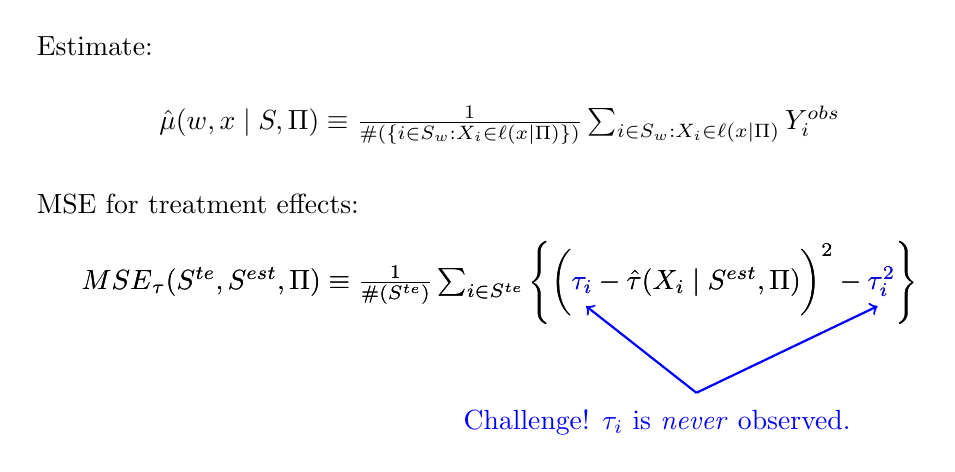
\begin{tikzpicture}
\node[anchor=west] at (-6,1) {Estimate:};
\onslide<1->{
\node at (0,0) {$\hat\mu(w,x\mid S,\Pi)\equiv \frac{1}{\# (\{i\in S_w:X_i\in\ell(x\mid\Pi)\})} \sum_{i\in S_w:X_i\in\ell(x\mid\Pi)}Y_i^\text{obs}$};
}
\onslide<2->{
\node[anchor=west] at (-6,-1) {MSE for treatment effects:};
\only<2-2>{
\node at (0,-2) {$\text{MSE}_\tau(S^\text{te},S^\text{est},\Pi)\equiv \frac{1}{\#(S^\text{te})}\sum_{i\in S^\text{te}}\Bigg\{\bigg(\tau_i-\hat\tau(X_i\mid S^\text{est},\Pi)\bigg)^2 - \tau_i^2\Bigg\}$};
}
\onslide<3-3>{
\node at (0,-2) {$\text{MSE}_\tau(S^\text{te},S^\text{est},\Pi)\equiv \frac{1}{\#(S^\text{te})}\sum_{i\in S^\text{te}}\Bigg\{\bigg(\blue{\tau_i}-\hat\tau(X_i\mid S^\text{est},\Pi)\bigg)^2 - \blue{\tau_i^2}\Bigg\}$};
\node[anchor=north,align=center,blue] at (2,-3.5) {Challenge! $\tau_i$ is \emph{never} observed.};
\draw[->, thick, blue] (2.5,-3.4) -- (1.1, -2.3);
\draw[->, thick, blue] (2.5,-3.4) -- (4.8, -2.3);
}
}
\end{tikzpicture}
\end{center}
\end{frame}

\begin{frame}{Adapt $\text{EMSE}_\mu$ to estimate $\text{EMSE}_\tau$}
\begin{center}
\begin{tikzpicture}
\node[anchor=north] at (0,0) {\scalebox{.8}{$\begin{aligned}
-\widehat{\text{EMSE}}_\mu (S^\text{tr},N^\text{est},\Pi) &= \underbrace{\frac{1}{N^\text{tr}} \sum_{i\in S^\text{tr}} \hat\mu^2(X_i\mid S^\text{tr},\Pi)}_\text{Conventional CART criterion} - \underbrace{\left(\frac{1}{N^\text{tr}} + \frac{1}{N^\text{est}}\right)\sum_{\ell\in\Pi}S^2_{S^\text{tr}}(\ell)}_\text{Uncertainty about leaf means}
\end{aligned}$}};
\node[anchor=north] at (0,-2) {\scalebox{.8}{$\begin{aligned}
-\widehat{\text{EMSE}}_\tau (S^\text{tr},N^\text{est},\Pi) &= \underbrace{\frac{1}{N^\text{tr}} \sum_{i\in S^\text{tr}} \hat\tau^2(X_i\mid S^\text{tr},\Pi)}_{\substack{\text{Variance of treatment}\\\text{effects across leaves}}} \\
&\qquad - \underbrace{\left(\frac{1}{N^\text{tr}} + \frac{1}{N^\text{est}}\right)\sum_{\ell\in\Pi}\bigg(\frac{S^2_{S^\text{tr}_\text{treat}}(\ell)}{p} + \frac{S^2_{S^\text{tr}_\text{control}}(\ell)}{1-p} \bigg)}_\text{Uncertainty about leaf treatment effects}
\end{aligned}$}};
\onslide<2-2>{
\node[align=center,blue] (het) at (-4,-4) {\footnotesize Prefers leaves with\\ \footnotesize heterogeneous effects};
\node[align=center,blue] (fit) at (-4,-6) {\footnotesize Prefers leaves with good fit\\ \footnotesize (leaf-specific effects\\ \footnotesize estimated precisely)};
\draw[->,thick,blue] (het) -- (-2,-3);
\draw[->,thick,blue] (fit) -- (-1,-5);
}
\end{tikzpicture}
\end{center}
\end{frame}

\begin{frame}
\huge Four partitioning estimators
\end{frame}

\begin{frame}{1. Causal trees}
Split by
\begin{center}
\begin{tikzpicture}
\node[anchor=north] at (0,-2) {\scalebox{.8}{$\begin{aligned}
-\widehat{\text{EMSE}}_\tau (S^\text{tr},N^\text{est},\Pi) &= \underbrace{\frac{1}{N^\text{tr}} \sum_{i\in S^\text{tr}} \hat\tau^2(X_i\mid S^\text{tr},\Pi)}_{\substack{\text{Variance of treatment}\\\text{effects across leaves}}} \\
&\qquad - \underbrace{\left(\frac{1}{N^\text{tr}} + \frac{1}{N^\text{est}}\right)\sum_{\ell\in\Pi}\bigg(\frac{S^2_{S^\text{tr}_\text{treat}}(\ell)}{p} + \frac{S^2_{S^\text{tr}_\text{control}}(\ell)}{1-p} \bigg)}_\text{Uncertainty about leaf treatment effects}
\end{aligned}$}};
\node[align=center,blue] (het) at (-4,-3.5) {\footnotesize Prefers leaves with\\ \footnotesize heterogeneous effects};
\node[align=center,blue] (fit) at (-4,-5) {\footnotesize Prefers leaves with good fit\\ \footnotesize (leaf-specific effects\\ \footnotesize estimated precisely)};
\draw[->,thick,blue] (het) -- (-2,-3);
\draw[->,thick,blue] (fit) -- (-1.2,-4.6);
\end{tikzpicture}
\end{center}
\begin{itemize}
\item \blue{Benefit}: Prioritizes heterogeneity ($\hat\tau$ varies a lot) and fit (within-leaf precision)
\item \blue{Drawback:} Cannot be done with off-the-shelf CART methods
\end{itemize}
\end{frame}

\begin{frame}{2. Transformed outcome trees}
Transform the outcome
$$Y_i^*=Y_i \frac{W_i-p}{p(1-p)}\rightarrow \E(Y_i^*\mid X_i=x) = \tau(x)$$
\begin{center}
\scalebox{.7}{$\begin{aligned}
\E(Y_i^*) &= \E\bigg[Y_i\frac{W_i-p}{p(1-p)}\bigg] \\
&= \E\bigg[Y_i\frac{W_i}{p(1-p)}\bigg] - \E\bigg[Y_i\frac{p}{p(1-p)}\bigg] \\
&= \E\bigg[Y_i(1)\frac{W_i}{p(1-p)}\bigg] - \E\bigg[\bigg(Y_i(1)W_i + Y_i(0)(1-W_i)\bigg)\frac{p}{p(1-p)}\bigg] \\
&= Y_i(1)\frac{1}{p(1-p)}\E[W_i] - Y_i(1)\frac{p}{p(1-p)}\E[W_i] - Y_i(0)\frac{p}{p(1-p)}\E[1-W_i] \\
&= Y_i(1)\frac{1-p}{p(1-p)}\E[W_i] - Y_i(0)\frac{p}{p(1-p)}\E[1-W_i] \\
&= Y_i(1)\frac{p(1-p)}{p(1-p)} - Y_i(0)\frac{p(1-p)}{p(1-p)} \\
&= Y_i(1) - Y_i(0) = \tau_i
\end{aligned}$}
\end{center}
\end{frame}

\begin{frame}{2. Transformed outcome trees}
\begin{itemize}
\item \blue{Benefit:} Can use off-the-shelf CART methods for prediction
\item \blue{Drawbacks:} Inefficient. Treatment is ignored after transforming outcome. \\
If within a leaf $\bar{W}\neq p$ (by chance), then sample average within leaf is a poor estimator of $\hat\tau$.
\end{itemize}
\end{frame}

\begin{frame}{3. Fit-based trees}
Replace
$$\text{MSE}_\mu(S^\text{te},S^\text{est},\Pi) \equiv \frac{1}{\#(S^\text{te})}\sum_{i\in S^\text{te}}\bigg\{(Y_i-\hat\mu(X_i;S^\text{est},\Pi))^2 - Y_i^2\bigg\}$$
with the fit-based split rule
$$\text{MSE}_{\mu,W}(S^\text{te},S^\text{est},\Pi) \equiv \sum_{i\in S^\text{te}}\bigg\{(Y_i-\hat\mu_w(W_iX_i;S^\text{est},\Pi))^2 - Y_i^2\bigg\}$$
which loss by \blue{model fit within each leaf}: the difference from the expected value for the treatment group of observation $i$. \vskip .2cm
\blue{Benefit:} Prefers splits that lead to better fit. \vskip .2cm
\blue{Drawback:} Does not prefer splits that lead to variation in treatment effects.
\myfootnote{Zeileis et al. 2008}
\end{frame}

\begin{frame}{4. Squared T-statistic trees}
Split based on:
\begin{center}
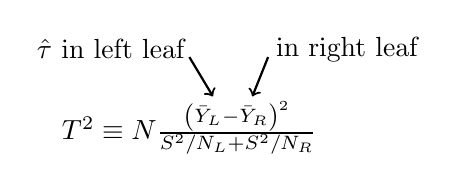
\begin{tikzpicture}
\node at (0,0) {$T^2\equiv N\frac{\left(\bar{Y}_L-\bar{Y}_R\right)^2}{S^2/N_L+S^2/N_R}$};
\node at (-1,1) {$\hat\tau$ in left leaf};
\node at (2,1) {in right leaf};
\draw[->,thick] (0,.9) -- (.3,.4);
\draw[->,thick] (1,.9) -- (.8,.4);
\end{tikzpicture}
\end{center}
\blue{Benefit:} Prefers splits that lead to variation in treatment effects. \vskip .2cm
\blue{Drawback:} Missed opportunity to improve fit: ignores useful splits between leaves with similar treatment effects but very different average values.
\myfootnote{Su et al. 2009}
\end{frame}

\begin{frame}{From trees to forests: Double-sample trees}

An individual tree can be noisy. Instead, we might fit a forest.

\begin{enumerate}
\item Draw a sample of size $s$
\item Split into an $\mathcal{I}$ and $\mathcal{J}$ sample.
\item Grow a tree on the $\mathcal{J}$ sample
\item Estimate leaf-specific $\hat\tau_\ell$ using the $\mathcal{I}$ sample
\end{enumerate}
Repeat many times. \vskip .5cm
\begin{columns}
\begin{column}{.5\textwidth}
\blue{Advantages of forests:}
\begin{itemize}
\item Consistent for true $\tau(x)$
\item Asymptotic normality
\item Asymptotic variance is estimable
\end{itemize}
\end{column}
\begin{column}{.5\textwidth}
\blue{Why \emph{double-sample} forests:}
\begin{itemize}
\item Advantage: Trees search for heterogeneous effects
\item Disadvantage: Requires sample splitting
\end{itemize}
\end{column}
\end{columns}

\myfootnote{Wager \& Athey 2017}
\end{frame}

\begin{frame}{From trees to forests: Propensity trees}

An individual tree can be noisy. Instead, we might fit a forest.

\begin{enumerate}
\item Draw a sample of size $s$
\item Grow a tree on the $\mathcal{J}$ sample to predict $W$
\begin{itemize}
\item[--] Each leaf must have at least $k$ observations of each treatment class
\end{itemize}
\item Estimate $\hat\tau_\ell$ on each leaf
\end{enumerate}
Repeat many times. \vskip .5cm
\begin{columns}
\begin{column}[t]{.5\textwidth}
\blue{Advantages of forests:}
\begin{itemize}
\item Consistent for true $\tau(x)$
\item Asymptotic normality
\item Asymptotic variance is estimable
\end{itemize}
\end{column}
\begin{column}[t]{.5\textwidth}
\blue{Why \emph{propensity} forests:}
\begin{itemize}
\item Advantage: Can use full sample
\item Disadvantage: Does not search for heterogeneous effects
\end{itemize}
\end{column}
\end{columns}

\myfootnote{Wager \& Athey 2017}
\end{frame}

\begin{frame}{Summary of causal trees and forests}
\begin{itemize}
\item There is no ground truth: We \blue{never observe $\tau_i$} \pause
\item Causal trees search for leaves with
\begin{itemize}
\item heterogeneous effects across leaves
\item precisely-estimated leaf effects
\end{itemize} \pause
\item Require extra \blue{sample splitting} \pause
\item Work well with randomized treatments. \pause
\item With selection on observables, the general recommendation is \blue{propensity forests}
\begin{itemize}
\item Maximizes the goal of \blue{addressing confounding} by ignoring \blue{heterogeneous effects} when choosing splits \pause
\item Generalized random forests also perform well {\footnotesize{(Athey, Tibshirani, \& Wager 2017)}} \pause
\item But ``the challenge in using adaptive methods\dots is that selection bias can be difficult to quantify'' {\footnotesize (Wager \& Athey p. 24)}.
\end{itemize}
\end{itemize}
\end{frame}

\begin{frame}{If treatment is \blue{not} randomized}
%Athey \& Imbens recommend:
%\begin{enumerate}
%\item Assume conditional ignorability: $\{Y_i(0),Y_i(1)\indep W_i\mid Z_i\}$
%\item Estimate $p_i=P(W_i\mid Z_i)$
%\item Reweight by normalized propensity score within each leaf
%\end{enumerate} \vskip 1cm
\begin{center}
\LARGE 
Causal trees find heterogeneous effects but \\
\blue{cannot guarantee that confounding is addressed.} \vskip 1cm
Next we focus on \\
\blue{why high-dimensional confounding is hard}
\end{center}
\end{frame}

\section{Regularization + confounding}

\begin{frame}{Why aren't causal trees guaranteed to address confounding?}
Plan
\begin{enumerate}
\item What does address confounding? \blue{Standardization}
\item Why is tree-based standardization biased? \blue{Regularization}
\item Is there anything we can do? \blue{Chernozhukov et al.}
\end{enumerate}
\end{frame}

\begin{frame}{What works: Nonparametric standardization}
\centering
\begin{tikzpicture}
\onslide<1-4>{
\node[anchor=north west] at (0,2.5) {What if $\{Y_i(0),Y_i(1)\}\not\indep W_i$ but $\{Y_i(0),Y_i(1)\}\indep W_i\mid X_i$?};
}
\onslide<4-4>{
\node[anchor=north west] at (0,1.5) {We need to estimate $\hat\tau$ \blue{within each level} of $X_i$.};
}
\onslide<2-5>{
\node[anchor=north west] at (0,0) {
\begin{scriptsize}
\begin{tabular}{cccccc}
& & & \multicolumn{2}{c}{Potential employment} & \\
\cmidrule(lr){4-5}
& Education & Treated & No job training & Job training & Treatment effect \\
ID & $X_i$ & $W_i$ & $Y_i(0)$ & $Y_i(1)$ & $\tau_i = Y_i(1) - Y_i(0)$ \\
\hline
1 & High school & 0 & 0 & \only<2-2>{1}\only<3->{?} & \only<2-2>{1}\only<3->{?} \\
2 & High school & 0 & 0 & \only<2-2>{1}\only<3->{?} & \only<2-2>{1}\only<3->{?} \\
3 & High school & 1 & \only<2-2>{0}\only<3->{?} & 1 & \only<2-2>{1}\only<3->{?} \\
4 & College &        0 & 1 & \only<2-2>{1}\only<3->{?} & \only<2-2>{0}\only<3->{?} \\
5 & College &        1 & \only<2-2>{1}\only<3->{?} & 1 & \only<2-2>{0}\only<3->{?} \\
6 & College &        1 & \only<2-2>{1}\only<3->{?} & 1 & \only<2-2>{0}\only<3->{?} \\
\end{tabular}
\end{scriptsize}
};
}
\onslide<5->{
\node[anchor = north west] at (0,3.5) {\scalebox{.8}{$\begin{aligned}
\hat{\bar\tau} &= \sum_{x\in\text{Support of }X} \P(X = x)\bigg(\bar{Y}_{i:W_i=1,X_i=x} - \bar{Y}_{i:W_i=0,X_i=x}\bigg)\\
&= \P(X_i=\text{High school})
\only<5,7->{\bigg(\bar{Y}_{i:W_i=1,X_i=\text{High school}} - \bar{Y}_{i:W_i=0,X_i=\text{High school}}\bigg)}
\only<6-6>{\blue{\bigg(\bar{Y}_{i:W_i=1,X_i=\text{High school}} - \bar{Y}_{i:W_i=0,X_i=\text{High school}}\bigg)}}
\\
&\qquad + \P(X_i=\text{College})
\only<5-6,8>{\bigg(\bar{Y}_{i:W_i=1,X_i=\text{College}} - \bar{Y}_{i:W_i=0,X_i=\text{College}}\bigg)}
\only<7-7>{\blue{\bigg(\bar{Y}_{i:W_i=1,X_i=\text{College}} - \bar{Y}_{i:W_i=0,X_i=\text{College}}\bigg)}}
\\
&= \frac{1}{2}\only<5,7->{(1 - 0)}\only<6-6>{\blue{(1-0)}} + \frac{1}{2}\only<5-6,8>{(1 - 1)}\only<7-7>{\blue{(1-1)}} = 0.5 + 0 = \only<--7>{0.5}\only<8-8>{\blue{0.5}}
\end{aligned}$}};
}
\only<6-6>{
\node[anchor=north west] at (0,0) {
\begin{scriptsize}
\begin{tabular}{cccccc}
& & & \multicolumn{2}{c}{Potential employment} & \\
\cmidrule(lr){4-5}
& Education & Treated & No job training & Job training & Treatment effect \\
ID & $X_i$ & $W_i$ & $Y_i(0)$ & $Y_i(1)$ & $\tau_i = Y_i(1) - Y_i(0)$ \\
\hline
\rowcolor{blue!10} 1 & High school & 0 & 0 & ? & ? \\
\rowcolor{blue!10} 2 & High school & 0 & 0 & ? & ? \\
\rowcolor{blue!10} 3 & High school & 1 & ? & 1 & ? \\
4 & College &        0 & 1 & ? & ? \\
5 & College &        1 & ? & 1 & ? \\
6 & College &        1 & ? & 1 & ? \\
\end{tabular}
\end{scriptsize}
};
}
\only<7-7>{
\node[anchor=north west] at (0,0) {
\begin{scriptsize}
\begin{tabular}{cccccc}
& & & \multicolumn{2}{c}{Potential employment} & \\
\cmidrule(lr){4-5}
& Education & Treated & No job training & Job training & Treatment effect \\
ID & $X_i$ & $W_i$ & $Y_i(0)$ & $Y_i(1)$ & $\tau_i = Y_i(1) - Y_i(0)$ \\
\hline
1 & High school & 0 & 0 & ? & ? \\
2 & High school & 0 & 0 & ? & ? \\
3 & High school & 1 & ? & 1 & ? \\
\rowcolor{blue!10} 4 & College &        0 & 1 & ? & ? \\
\rowcolor{blue!10} 5 & College &        1 & ? & 1 & ? \\
\rowcolor{blue!10} 6 & College &        1 & ? & 1 & ? \\
\end{tabular}
\end{scriptsize}
};
}
\only<8-8>{
\node[anchor=north west] at (0,0) {
\begin{scriptsize}
\begin{tabular}{cccccc}
& & & \multicolumn{2}{c}{Potential employment} & \\
\cmidrule(lr){4-5}
& Education & Treated & No job training & Job training & Treatment effect \\
ID & $X_i$ & $W_i$ & $Y_i(0)$ & $Y_i(1)$ & $\tau_i = Y_i(1) - Y_i(0)$ \\
\hline
\rowcolor{blue!10} 1 & High school & 0 & 0 & ? & ? \\
\rowcolor{blue!10} 2 & High school & 0 & 0 & ? & ? \\
\rowcolor{blue!10} 3 & High school & 1 & ? & 1 & ? \\
\rowcolor{blue!10} 4 & College &        0 & 1 & ? & ? \\
\rowcolor{blue!10} 5 & College &        1 & ? & 1 & ? \\
\rowcolor{blue!10} 6 & College &        1 & ? & 1 & ? \\
\end{tabular}
\end{scriptsize}
};
}
\end{tikzpicture}
\end{frame}

\begin{frame}{What works: Nonparametric standardization}
\centering
\Large But when there are \blue{many cells} of the covariates $X_i$, \vskip 1cm
{\huge nonparametric standardization is \blue{impossible}!}
\end{frame}

\begin{frame}{Why is tree-based standardization biased? \blue{Regularization}}
With no regularization, a tree would grow until each leaf was completely homogenous in $X_i$. \vskip 1cm
But this tree would be very noisy! We prune our trees so that leaves contain more observations.
\begin{itemize}
\item Treatment effects are more \blue{precisely estimated}
\item But treatment effects are \blue{biased} if there is confounding within leaves
\end{itemize}
\end{frame}

\begin{frame}{Is there anything we can do? \blue{Chernozhukov et al.}}
$$\overbrace{Y = D\theta_0 + g_0(X) + U}^\text{Outcome equation}\qquad \overbrace{D = m_0(X) + V}^\text{Treatment assignment}$$
One might be tempted to estimate $\hat{g}_0(X)$ by machine learning and then state:
$$\hat\theta_0 = \frac{
\frac{1}{n}\sum_{i\in\mathcal{I}}D_i(Y_i-\hat{g}_0(X_i))
}{
\frac{1}{n}\sum_{i\in\mathcal{I}}D_i^2
}$$ \pause
This will be \blue{biased} because the estimator $\hat{g}_0$ is \blue{regularized}.
$$b = \frac{1}{\E(D_i^2)}\frac{1}{\sqrt{n}}\sum_{i\in\mathcal{I}}\overbrace{\bigg(m_0(X_i)(g_0(X_i) - \hat{g}_0(X_i)\bigg)}^\text{Does not have mean 0} + o_P(1)$$ \pause
\blue{Key:} $D_i$ is centered at $m_0(X)\neq 0$. We should \blue{recenter $D_i$}.
\end{frame}

\begin{frame}{Is there anything we can do? \blue{Chernozhukov et al.}}
$$\overbrace{Y = D\theta_0 + g_0(X) + U}^\text{Outcome equation}\qquad \overbrace{D = m_0(X) + V}^\text{Treatment assignment}$$
\begin{enumerate}
\item Split the sample into $\mathcal{I}$ and $\mathcal{J}$
\item Estimate $\hat{g}_0(X)$ using sample $\mathcal{J}$
\item Estimate $\hat{m}_0(X)$ using sample $\mathcal{J}$
\item Orthogonalize $D$ on $X$ (approximately)
$$\hat{V} = D - \hat{m}_0(X)$$
\item Estimate the treatment effect
\end{enumerate}
\begin{tabular}{>{\centering\arraybackslash}p{.5\textwidth}>{\centering\arraybackslash}p{.5\textwidth}}
\blue{Biased} & \blue{De-biased} \\
$\hat\theta_0 = \frac{
\frac{1}{n}\sum_{i\in\mathcal{I}}D_i(Y_i-\hat{g}_0(X_i))
}{
\frac{1}{n}\sum_{i\in\mathcal{I}}D_i^2
}$
&
$\hat\theta_0 = \frac{
\frac{1}{n}\sum_{i\in\mathcal{I}}\hat{V}_i(Y_i-\hat{g}_0(X_i))
}{
\frac{1}{n}\sum_{i\in\mathcal{I}}\hat{V}_iD_i
}$
\end{tabular}

\myfootnote{Chernozhukov et al. 2016}
\end{frame}

\begin{frame}[t]{Bias remaining in de-biased estimator {\scriptsize (Chernozhukov et al.)}}
$$\sqrt{n}(\hat\theta_0 - \theta_0) = a^* + b^* + c^*$$
\only<2-2>{
$$a^*=\frac{1}{\E(V^2)}\frac{1}{\sqrt{n}}\sum_{i\in\mathcal{I}}V_iU_i\rightarrow N(0,\Sigma)$$
Because $a^*$ converges to mean 0, we don't worry about it. \\
}
\only<3-3>{
Regularization bias:
$$b^* =\frac{1}{\E(V^2)}\frac{1}{\sqrt{n}}\sum_{i\in\mathcal{I}}\bigg(\hat{m}_0(X_i)-m_0(X_i)\bigg)\bigg(\hat{g}_0(X_i)-g_0(X_i)\bigg)$$
Vanishes ``under a broad range of data-generating processes.'' \vskip .5cm
Bounded above by
\begin{center}
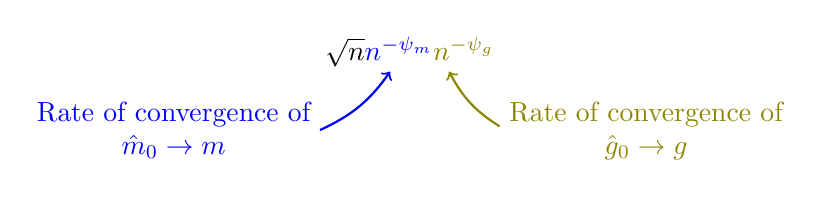
\begin{tikzpicture}
\node[align=center, blue] (mConv) at (-3,-1) {Rate of convergence of\\$\hat{m}_0\rightarrow m$};
\node[align=center, olive] (gConv) at (3,-1) {Rate of convergence of\\$\hat{g}_0\rightarrow g$};
\node at (0,0) {$\sqrt{n}\blue{n^{-\psi_m}}\green{n^{-\psi_g}}$};
\draw[->, thick, blue] (mConv) to[bend right=15] (-.25,-.25);
\draw[->, thick, olive] (gConv) to[bend left=15] (.5,-.25);
\end{tikzpicture}
\end{center}
}
\only<4-4>{
An example of the third term in the partially linear model:
$$c^*=\frac{1}{\sqrt{n}}\sum_{i\in\mathcal{I}} V_i\bigg(\hat{g}_0(X_i) - g_0(X_i)\bigg)$$
If $\hat{g}_0$ is estimated on an \blue{auxiliary sample} $\mathcal{J}$, then $V_i$ and $\hat{g}_0(X_i)$ will be uncorrelated and $\E(c^*)=0$.
}
\end{frame}

\section{BART}

\begin{frame}{BART: Bayesian Additive Regression Trees}

Differs from random forests:
\begin{itemize}
\item Fixed number of trees
\item Backfits repeatedly over the fixed number of trees
\item Strong prior encourages shallow trees
\item Uncertainty comes automatically from posterior samples
\end{itemize}

\myfootnote{Chipman, George, \& McCulloch 2010}
\end{frame}

\begin{frame}{BART model}
\begin{center}
\scalebox{.6}{$\begin{aligned}
Y &= \sum_{j=1}^m g_j(x\mid T_j,M_j) + \epsilon \\
\epsilon &\sim N(0,\sigma^2) \\
\blue{\blue{T_j\text{ prior}}}& \\
P(\underbrace{D_j=d}_\text{Tree depth}) &= \alpha(1+d)^{-\beta} \\
\text{Split variable} &\sim \text{Uniform}(\text{Available variables}) \\
\text{Split value} &\sim \text{Uniform}(\text{Available split values}) \\
\blue{\mu_{ij}\mid T_j \text{ prior}}& \\
\underbrace{\mu_{ij}}_{\text{Tree }i\text{ leaf }j}&\sim N\bigg(\underbrace{\mu_m,\sigma^2_\mu}_{\substack{\text{Chosen so that}\\\text{high probability of}\\E(Y\mid x)\in(y_\text{min},y_\text{max})}}\bigg) \\
\blue{\sigma\text{ prior}}& \\
\sigma &\sim \frac{\nu\lambda}{\chi^2_\nu}\text{ (inverse chi-square)}
\end{aligned}$}
\end{center}
They recommend $\{\alpha = .95, \beta=2\} \rightarrow$ 97\% of prior probability is on 4 or fewer terminal nodes.

\myfootnote{Chipman, George, \& McCulloch 2010}
\end{frame}

\begin{frame}{BART for causal inference}
\blue{Goal}: Model the \blue{response surface} as a function of treatment and pre-treatment covariates
\begin{enumerate}
\item Fit a flexible model for $Y = f(X,W)$
\item Set $W = 0$ to predict $\hat{Y}_i(0)$ for all $i$
\item Set $W = 1$ to predict $\hat{Y}_i(1)$ for all $i$
\item Difference to estimate $\hat\tau_i$
\item Plot effects
\end{enumerate}
\begin{center}
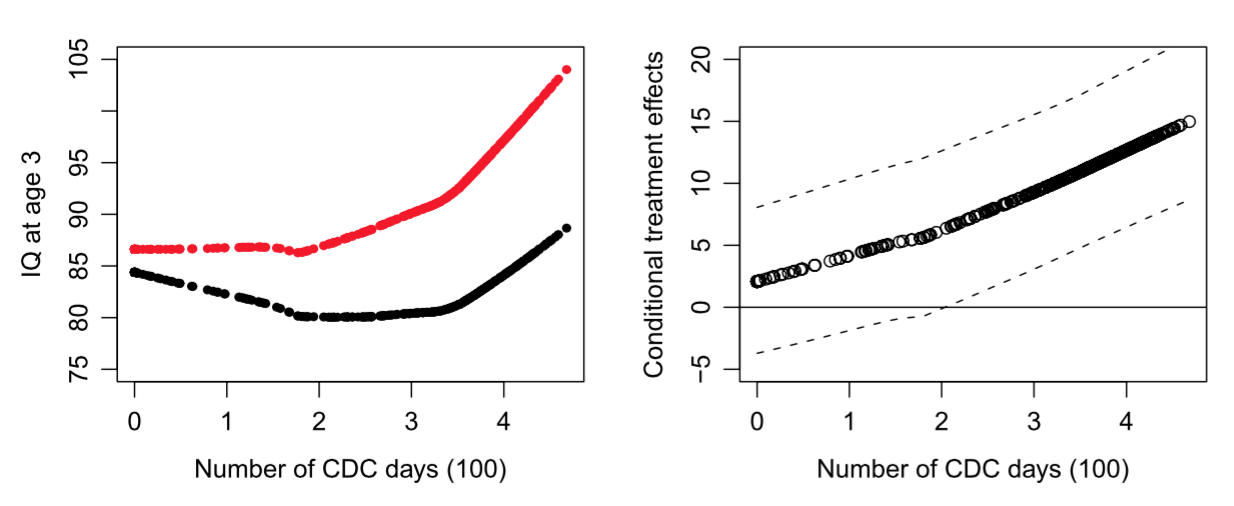
\includegraphics[width = .7\textwidth]{figures/HillFigure}
\end{center}
\myfootnote{Hill 2011}
\end{frame}

\begin{frame}{BART: Benefits and drawbacks}
Benefits
\begin{itemize}
\item Less researcher discretion for tuning parameters
\item Automatic posterior uncertainty estimates
\end{itemize}
Drawbacks
\begin{itemize}
\item Not guaranteed to address confounding due to regularization
\item No theoretical guarantees of centering over truth
\item Splitting is based on prediction and is not explicitly optimized for causal inference within leaves
\end{itemize}
\end{frame}

\begin{frame}{Summary}
\begin{itemize}
\item Causal trees can detect high-dimensional covariate-based treatment \blue{effect heterogeneity}
\item Work well with high-order interactions
\item Causal forests give theoretically valid \blue{confidence intervals}
\item Bayesian approaches (BART) are less theoretically verified but give easy uncertainty
\item With high-dimensional \blue{confounding}, all methods are biased but can be designed to be consistent.
\end{itemize}
\end{frame}

\end{document}

\begin{frame}{Standardization}
\begin{footnotesize}
\begin{tabular}{cccccc}
& & & \multicolumn{2}{c}{Potential employment} & \\
\cmidrule(lr){4-5}
& Education & Treated & No job training & Job training & Treatment effect \\
ID & $X_i$ & $W_i$ & $Y_i(0)$ & $Y_i(1)$ & $\tau_i = Y_i(1) - Y_i(0)$ \\
\hline
1 & High school & 0 & 0 & ? & ? \\
2 & High school & 0 & 0 & ? & ? \\
3 & High school & 1 & ? & 1 & ? \\
4 & College &        0 & 1 & ? & ? \\
5 & College &        1 & ? & 1 & ? \\
6 & College &        1 & ? & 1 & ? \\
\end{tabular} \\ \pause
$$\begin{aligned}
\hat{\bar\tau} &= \P(X_i=\text{High school})\bigg(\bar{Y}_{i:W_i=1,X_i=\text{High school}} - \bar{Y}_{i:W_i=0,X_i=\text{High school}}\bigg) \\
&\qquad + \P(X_i=\text{College})\bigg(\bar{Y}_{i:W_i=1,X_i=\text{College}} - \bar{Y}_{i:W_i=0,X_i=\text{College}}\bigg) \\
&= \frac{1}{2}(1 - 0) + \frac{1}{2}(1 - 1) = 0.5 + 0 = 0.5
\end{aligned}$$
\end{footnotesize}
\myfootnote{Hernan \& Robins manuscript, p. 18}
\end{frame}

\begin{frame}{Standardization}
\begin{footnotesize}
\begin{tabular}{cccccc}
& & & \multicolumn{2}{c}{Potential employment} & \\
\cmidrule(lr){4-5}
& Education & Treated & No job training & Job training & Treatment effect \\
ID & $X_i$ & $W_i$ & $Y_i(0)$ & $Y_i(1)$ & $\tau_i = Y_i(1) - Y_i(0)$ \\
\hline
1 & High school & 0 & 0 & ? & ? \\
2 & High school & 0 & 0 & ? & ? \\
3 & High school & 1 & ? & 1 & ? \\
4 & College &        0 & 1 & ? & ? \\
5 & College &        1 & ? & 1 & ? \\
6 & College &        1 & ? & 1 & ? \\
\end{tabular} \\
$$\begin{aligned}
\hat{\bar\tau} &= \sum_{x\in\text{ Support of }X} \P(X_i=x)\bigg(\bar{Y}_{i:W_i=1,X_i=x} - \bar{Y}_{i:W_i=0,X_i=x}\bigg) \\
&= \frac{1}{2}(1 - 0) + \frac{1}{2}(1 - 1) = 0.5 + 0 = 0.5
\end{aligned}$$
\end{footnotesize}
\myfootnote{Hernan \& Robins manuscript, p. 18}
\end{frame}

\begin{frame}{Parametric g-formula}
\begin{footnotesize}
\begin{tabular}{cccccc}
& & & \multicolumn{2}{c}{Potential employment} & \\
\cmidrule(lr){4-5}
& Education & Treated & No job training & Job training & Treatment effect \\
ID & $X_i$ & $W_i$ & $Y_i(0)$ & $Y_i(1)$ & $\tau_i = Y_i(1) - Y_i(0)$ \\
\hline
1 & High school & 0 & 0 & ? & ? \\
2 & High school & 0 & 0 & ? & ? \\
3 & High school & 1 & ? & 1 & ? \\
4 & College &        0 & 1 & ? & ? \\
5 & College &        1 & ? & 1 & ? \\
6 & College &        1 & ? & 1 & ? 
\end{tabular} \vskip .3cm
$$\begin{aligned}
\hat{\bar\tau} &= \frac{1}{n}\sum \bigg(\hat{Y}_i(1) - \hat{Y}_i(0)\bigg)
\end{aligned}$$
\end{footnotesize}
\myfootnote{Hernan \& Robins manuscript, Part II, p. 24}
\end{frame}

\begin{frame}{Parametric g-formula}
\begin{footnotesize}
\begin{tabular}{cccccc}
& & & \multicolumn{2}{c}{Potential employment} & \\
\cmidrule(lr){4-5}
& Education & Treated & No job training & Job training & Treatment effect \\
ID & $X_i$ & $W_i$ & $Y_i(0)$ & $Y_i(1)$ & $\tau_i = Y_i(1) - Y_i(0)$ \\
\hline
\rowcolor{blue!10} 1 & High school & 0 & 0 & ? & ? \\
\rowcolor{blue!10} 2 & High school & 0 & 0 & ? & ? \\
3 & High school & 1 & ? & 1 & ? \\
\rowcolor{blue!10} 4 & College &        0 & 1 & ? & ? \\
5 & College &        1 & ? & 1 & ? \\
6 & College &        1 & ? & 1 & ? 
\end{tabular} \vskip .3cm
1. Fit a model $\hat{Y}=f_0(X)$ among the control observations.
\end{footnotesize}
\myfootnote{Hernan \& Robins manuscript, Part II, p. 24}
\end{frame}

\begin{frame}{Parametric g-formula}
\begin{footnotesize}
\begin{tabular}{cccccc}
& & & \multicolumn{2}{c}{Potential employment} & \\
\cmidrule(lr){4-5}
& Education & Treated & No job training & Job training & Treatment effect \\
ID & $X_i$ & $W_i$ & $Y_i(0)$ & $Y_i(1)$ & $\tau_i = Y_i(1) - Y_i(0)$ \\
\hline
1 & High school & 0 & \cellcolor{blue!10}0 & ? & ? \\
2 & High school & 0 & \cellcolor{blue!10}0 & ? & ? \\
3 & High school & 1 & \cellcolor{blue!10}? & 1 & ? \\
4 & College &        0 & \cellcolor{blue!10}1 & ? & ? \\
5 & College &        1 & \cellcolor{blue!10}? & 1 & ? \\
6 & College &        1 & \cellcolor{blue!10}? & 1 & ? 
\end{tabular} \vskip .3cm
2. Impute the potential outcome under control.
\end{footnotesize}
\myfootnote{Hernan \& Robins manuscript, Part II, p. 24}
\end{frame}

\begin{frame}{Parametric g-formula}
\begin{footnotesize}
\begin{tabular}{cccccc}
& & & \multicolumn{2}{c}{Potential employment} & \\
\cmidrule(lr){4-5}
& Education & Treated & No job training & Job training & Treatment effect \\
ID & $X_i$ & $W_i$ & $\hat{Y}_i(0)$ & $Y_i(1)$ & $\tau_i = Y_i(1) - Y_i(0)$ \\
\hline
1 & High school & 0 & \cellcolor{blue!10}0 & ? & ? \\
2 & High school & 0 & \cellcolor{blue!10}0 & ? & ? \\
3 & High school & 1 & \cellcolor{blue!10}0 & 1 & ? \\
4 & College &        0 & \cellcolor{blue!10}1 & ? & ? \\
5 & College &        1 & \cellcolor{blue!10}1 & 1 & ? \\
6 & College &        1 & \cellcolor{blue!10}1 & 1 & ? 
\end{tabular} \vskip .3cm
2. Impute the potential outcome under control.
\end{footnotesize}
\myfootnote{Hernan \& Robins manuscript, Part II, p. 24}
\end{frame}

\begin{frame}{Parametric g-formula}
\begin{footnotesize}
\begin{tabular}{cccccc}
& & & \multicolumn{2}{c}{Potential employment} & \\
\cmidrule(lr){4-5}
& Education & Treated & No job training & Job training & Treatment effect \\
ID & $X_i$ & $W_i$ & $\hat{Y}_i(0)$ & $Y_i(1)$ & $\tau_i = Y_i(1) - Y_i(0)$ \\
\hline
1 & High school & 0 & 0 & ? & ? \\
2 & High school & 0 & 0 & ? & ? \\
\rowcolor{blue!10} 3 & High school & 1 & 0 & 1 & ? \\
4 & College &        0 & 1 & ? & ? \\
\rowcolor{blue!10} 5 & College &        1 & 1 & 1 & ? \\
\rowcolor{blue!10} 6 & College &        1 & 1 & 1 & ? 
\end{tabular} \vskip .3cm
3. Fit a model $\hat{Y}=f_1(X)$ among the treated observations.
\end{footnotesize}
\myfootnote{Hernan \& Robins manuscript, Part II, p. 24}
\end{frame}

\begin{frame}{Parametric g-formula}
\begin{footnotesize}
\begin{tabular}{cccccc}
& & & \multicolumn{2}{c}{Potential employment} & \\
\cmidrule(lr){4-5}
& Education & Treated & No job training & Job training & Treatment effect \\
ID & $X_i$ & $W_i$ & $\hat{Y}_i(0)$ & $\hat{Y}_i(1)$ & $\tau_i = Y_i(1) - Y_i(0)$ \\
\hline
1 & High school & 0 & 0 & \cellcolor{blue!10}? & ? \\
2 & High school & 0 & 0 & \cellcolor{blue!10}? & ? \\
3 & High school & 1 & 0 & \cellcolor{blue!10}1 & ? \\
4 & College &        0 & 1 & \cellcolor{blue!10}? & ? \\
5 & College &        1 & 1 & \cellcolor{blue!10}1 & ? \\
6 & College &        1 & 1 & \cellcolor{blue!10}1 & ? 
\end{tabular} \vskip .3cm
4. Impute the potential outcome under treatment.
\end{footnotesize}
\myfootnote{Hernan \& Robins manuscript, Part II, p. 24}
\end{frame}

\begin{frame}{Parametric g-formula}
\begin{footnotesize}
\begin{tabular}{cccccc}
& & & \multicolumn{2}{c}{Potential employment} & \\
\cmidrule(lr){4-5}
& Education & Treated & No job training & Job training & Treatment effect \\
ID & $X_i$ & $W_i$ & $\hat{Y}_i(0)$ & $\hat{Y}_i(1)$ & $\tau_i = Y_i(1) - Y_i(0)$ \\
\hline
1 & High school & 0 & 0 & \cellcolor{blue!10}1 & ? \\
2 & High school & 0 & 0 & \cellcolor{blue!10}1 & ? \\
3 & High school & 1 & 0 & \cellcolor{blue!10}1 & ? \\
4 & College &        0 & 1 & \cellcolor{blue!10}1 & ? \\
5 & College &        1 & 1 & \cellcolor{blue!10}1 & ? \\
6 & College &        1 & 1 & \cellcolor{blue!10}1 & ? 
\end{tabular} \vskip .3cm
4. Impute the potential outcome under treatment.
\end{footnotesize}
\myfootnote{Hernan \& Robins manuscript, Part II, p. 24}
\end{frame}

\begin{frame}{Parametric g-formula}
\begin{footnotesize}
\begin{tabular}{cccccc}
& & & \multicolumn{2}{c}{Potential employment} & \\
\cmidrule(lr){4-5}
& Education & Treated & No job training & Job training & Treatment effect \\
ID & $X_i$ & $W_i$ & $\hat{Y}_i(0)$ & $\hat{Y}_i(1)$ & $\tau_i = Y_i(1) - Y_i(0)$ \\
\hline
1 & High school & 0 & 0 & 1 & \cellcolor{blue!10}? \\
2 & High school & 0 & 0 & 1 & \cellcolor{blue!10}? \\
3 & High school & 1 & 0 & 1 & \cellcolor{blue!10}? \\
4 & College &        0 & 1 & 1 & \cellcolor{blue!10}? \\
5 & College &        1 & 1 & 1 & \cellcolor{blue!10}? \\
6 & College &        1 & 1 & 1 & \cellcolor{blue!10}? 
\end{tabular} \vskip .3cm
5. Impute the treatment effect for each observation $i$
\end{footnotesize}
\myfootnote{Hernan \& Robins manuscript, Part II, p. 24}
\end{frame}

\begin{frame}{Parametric g-formula}
\begin{footnotesize}
\begin{tabular}{cccccc}
& & & \multicolumn{2}{c}{Potential employment} & \\
\cmidrule(lr){4-5}
& Education & Treated & No job training & Job training & Treatment effect \\
ID & $X_i$ & $W_i$ & $\hat{Y}_i(0)$ & $\hat{Y}_i(1)$ & $\hat\tau_i = \hat{Y}_i(1) - \hat{Y}_i(0)$ \\
\hline
1 & High school & 0 & 0 & 1 & \cellcolor{blue!10}1 \\
2 & High school & 0 & 0 & 1 & \cellcolor{blue!10}1 \\
3 & High school & 1 & 0 & 1 & \cellcolor{blue!10}1 \\
4 & College &        0 & 1 & 1 & \cellcolor{blue!10}0 \\
5 & College &        1 & 1 & 1 & \cellcolor{blue!10}0 \\
6 & College &        1 & 1 & 1 & \cellcolor{blue!10}0 
\end{tabular}  \vskip .3cm
5. Impute the treatment effect for each observation $i$
\end{footnotesize}
\myfootnote{Hernan \& Robins manuscript, Part II, p. 24}
\end{frame}

\begin{frame}{Parametric g-formula}
\begin{footnotesize}
\begin{tabular}{cccccc}
& & & \multicolumn{2}{c}{Potential employment} & \\
\cmidrule(lr){4-5}
& Education & Treated & No job training & Job training & Treatment effect \\
ID & $X_i$ & $W_i$ & $\hat{Y}_i(0)$ & $\hat{Y}_i(1)$ & $\hat\tau_i = \hat{Y}_i(1) - \hat{Y}_i(0)$ \\
\hline
1 & High school & 0 & 0 & 1 & 1 \\
2 & High school & 0 & 0 & 1 & 1 \\
3 & High school & 1 & 0 & 1 & 1 \\
4 & College &        0 & 1 & 1 & 0 \\
5 & College &        1 & 1 & 1 & 0 \\
6 & College &        1 & 1 & 1 & 0 
\end{tabular} \vskip .3cm
6. Average over the sample: \colorbox{blue!10}{$\hat{\bar\tau} = \frac{1}{n}\sum \hat\tau_i = \frac{1}{6}(3) = 0.5$}
\end{footnotesize}
\myfootnote{Hernan \& Robins manuscript, Part II, p. 24}
\end{frame}

\begin{frame}
In the example above, \vskip .2cm
\begin{center}
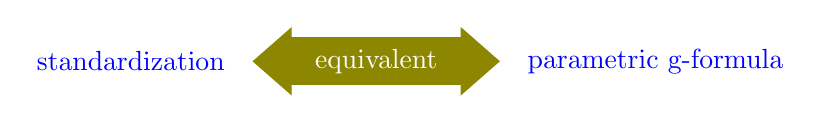
\begin{tikzpicture}[x=1.2cm,y=.3cm]
\node[anchor=east] at (-1.5, 0) {\blue{standardization}};
\node[anchor=west] at (1.5, 0) {\blue{parametric g-formula}};
\draw[fill=olive,color=olive] (1,1) -- (1,-1) -- (-1,-1) -- (-1,1) -- cycle;
\draw[fill=olive,color=olive] (1.3,0) -- (.9,1.4) -- (.9,-1.4) -- cycle;
\draw[fill=olive,color=olive] (-1.3,0) -- (-.9,1.4) -- (-.9,-1.4) -- cycle;
\node at (0,0) {\textcolor{white}{equivalent}};
\end{tikzpicture}
\end{center} \vskip .2cm
because the model was saturated. \vskip .5cm
In higher-dimension cases, standardization is impossible, \vskip .3cm
the two are not equivalent, \vskip .3cm
and \blue{parametric} assumptions matter.
\end{frame}

\begin{frame}{Parametric g-formula}
\begin{footnotesize}
\begin{tabular}{cccccc}
& & & \multicolumn{2}{c}{Potential employment} & \\
\cmidrule(lr){4-5}
& Education & Treated & No job training & Job training & Treatment effect \\
ID & $X_i$ & $W_i$ & $Y_i(0)$ & $Y_i(1)$ & $\tau_i = Y_i(1) - Y_i(0)$ \\
\hline
1 & 12 & 0 & 0 & ? & ? \\
2 & 13 & 0 & 0 & ? & ? \\
3 & 14 & 1 & ? & 1 & ? \\
4 & 16 &        0 & 1 & ? & ? \\
5 & 17 &        1 & ? & 1 & ? \\
6 & 18 &        1 & ? & 1 & ? 
\end{tabular} \vskip .3cm
$$\begin{aligned}
\hat{\bar\tau} &= \frac{1}{n}\sum \bigg(\hat{Y}_i(1) - \hat{Y}_i(0)\bigg)
\end{aligned}$$
\end{footnotesize} \\
Standardization is \blue{impossible}
\myfootnote{Hernan \& Robins manuscript, Part II, p. 24}
\end{frame}

\begin{frame}{Assume a parametric model}
Assume a \blue{partition}
$$\Pi = \bigg\{\ell_1=\{X < 16\},\ell_2=\{X\geq 16\}\bigg\}$$
Define a \blue{conditional mean function}
$$\mu(x\mid \Pi) \equiv \overbrace{\E\bigg[Y_i\mid \underbrace{X_i\in \ell(x\mid \Pi)}_\text{Within the leaf containing $x$}\bigg]}^\text{Piecewise constant function}$$
Use this parametric model to estimate the potential outcomes as \blue{piecewise constant} functions of education.
\end{frame}

\begin{frame}{Parametric g-formula}
\begin{footnotesize}
\begin{tabular}{cccccc}
& & & \multicolumn{2}{c}{Potential employment} & \\
\cmidrule(lr){4-5}
& Education & Treated & No job training & Job training & Treatment effect \\
ID & $X_i$ & $W_i$ & $Y_i(0)$ & $Y_i(1)$ & $\tau_i = Y_i(1) - Y_i(0)$ \\
\hline
1 & 12 & 0 & 0 & ? & ? \\
2 & 13 & 0 & 0 & ? & ? \\
3 & 14 & 1 & ? & 1 & ? \\
4 & 16 &        0 & 1 & ? & ? \\
5 & 17 &        1 & ? & 1 & ? \\
6 & 18 &        1 & ? & 1 & ? 
\end{tabular} \vskip .3cm
$$\begin{aligned}
\hat{\bar\tau} &= \frac{1}{n}\sum \bigg(\hat{Y}_i(1) - \hat{Y}_i(0)\bigg)
\end{aligned}$$ \pause 
$$\hat{Y}(1,x) = \hat\mu_1(x\mid \Pi) \equiv \E\bigg[Y_i\mid X_i\in \ell(x\mid \Pi)\bigg]$$
$$\hat{Y}(0,x) = \hat\mu_0(x\mid \Pi) \equiv \E\bigg[Y_i\mid X_i\in \ell(x\mid \Pi)\bigg]$$
\end{footnotesize}
\myfootnote{Hernan \& Robins manuscript, Part II, p. 24}
\end{frame}

\begin{frame}{Parametric g-formula}
\begin{footnotesize}
\begin{tabular}{cccccc}
& & & \multicolumn{2}{c}{Potential employment} & \\
\cmidrule(lr){4-5}
& Education & Treated & No job training & Job training & Treatment effect \\
ID & $X_i$ & $W_i$ & $Y_i(0)$ & $Y_i(1)$ & $\tau_i = Y_i(1) - Y_i(0)$ \\
\hline
1 & High school & 0 & 0 & ? & ? \\
2 & High school & 0 & 0 & ? & ? \\
3 & High school & 1 & ? & 1 & ? \\
4 & College &        0 & 1 & ? & ? \\
5 & College &        1 & ? & 1 & ? \\
6 & College &        1 & ? & 1 & ? 
\end{tabular} \vskip .3cm
$$\begin{aligned}
\hat{\bar\tau} &= \frac{1}{n}\sum \bigg(\hat{Y}_i(1) - \hat{Y}_i(0)\bigg)
\end{aligned}$$
$$\hat{Y}(1,x) = \hat\mu_1(x\mid \Pi) \equiv \E\bigg[Y_i\mid X_i\in \ell(x\mid \Pi)\bigg]$$
$$\hat{Y}(0,x) = \hat\mu_0(x\mid \Pi) \equiv \E\bigg[Y_i\mid X_i\in \ell(x\mid \Pi)\bigg]$$
\end{footnotesize}
\myfootnote{Hernan \& Robins manuscript, Part II, p. 24}
\end{frame}

\begin{frame}
This should feel familiar\dots \vskip .5cm \pause
it is effectively \blue{coarsened exact matching}. \vskip .5cm \pause
But the validity of inference now relies on parametric assumptions. \vskip .5cm \pause
Can an \blue{algorithm choose the partition} for coarsening?
\myfootnote{Iacus, King, \& Porro 2012}
\end{frame}

